\section{Performance Evaluation}
\label{sec:performance_evaluation}

In this section, we study the different strategies for improving SR through simulations. We use Komondor~\cite{barrachina2019komondor}, an IEEE 802.11 simulator with embedded AI-capable agents. The various MAB implementations were simulated along with the network operation using the parameters collected in Table~\ref{tbl:simulation_parameters}. More details on the considered IEEE 802.11 frame types, sizes, and inter-frame periods are in~\cite[Table~B.6]{wilhelmi2021spatial}.

\begin{table}[ht!]
\centering
\caption{Simulation parameters.}
\label{tbl:simulation_parameters}
\resizebox{.92\columnwidth}{!}{%
\begin{tabular}{@{}clc@{}}
\toprule
Parameter & \multicolumn{1}{c}{\textbf{Description}} & \textbf{Value} \\ \midrule
$t$ & Simulation time & $300$ s \\
%$N_\text{sim}$ & Number of random deployments & 100 \\
%$N_\text{BSS}$ & Number of BSSs & $1-9$ \\
$F_c$ & Carrier frequency & $5$ GHz \\
$\text{GI}$ & Guard Interval & $3.2$ $\mu$s\\ 
$B$ & Transmission bandwidth & $20$ MHz \\
$\text{MCS}$ & MCS indices & 0-11\\ 
$\mathcal{P}^\text{Noise}$ & Noise power & $-95$ dBm \\
$\mathcal{P}_{tx,\max}$ & Default transmit power & $20$ dBm \\
CCA & Default CCA threshold & $-82$ dBm \\
$S$ & Single-user spatial streams & $1$ \\
$G^\text{TX/RX}$ & Transmitter/receiver antenna gain & $0/0$ dBi \\
$\textrm{CE}$ & Capture effect threshold & $10$ dB \\
PL & Path loss model & See \cite{wilhelmi2021spatial} \\
$PL_0$ & Loss at the reference dist. & $5$ dB \\
$\nu$ & Path-loss exponent & $4.4$ \\
$\sigma$ & Shadowing factor & $9.5$ dB\\
$\omega$ & Obstacles factor & $30$ dB\\
$\text{TXOP}_{\max}$ & TXOP duration limit & $5.484$ ms\\ 
$\text{A-MPDU}_{\max}$ & A-MPDU size & $64$\\ 
$L_{D}$ & Length of data packets & $1500$ bytes \\ 
$\mathcal{T}$ & Traffic model & Full-buffer\\ 
$\mathbb{T}$ & Traffic type & Downlink (DL) \\ 
$\text{CW}_0$ & Initial Contention Window (CW) & $16$ \\
$\text{CWE}_{\min/\max}$ & Min./Max. CW exponent & $1/5$ \\
\midrule
$\gamma$ & PD values & $\{-72, -82\}$~dBm\\
$\zeta$ & Transmit power values & $\{10, 20\}$~dBm\\
$\Delta$ & Iteration duration & $0.5$~s \\
$\varepsilon_0$ & Initial exploration coefficient & $0.1$ \\
$\varepsilon(t)$ & Exploration coefficient & $\varepsilon_0/\sqrt{t}$ \\
\bottomrule
\end{tabular}%
}
\end{table}

\subsection{Interactions between 2 BSSs}

We start with the deployment depicted in Figure~\ref{fig:toy_scenario} (later referred to as the \textit{toy scenario}), which contains two BSSs where different contention and interference interactions occur depending on the power and PD used by the BSSs. To keep complexity low and clearly devise the effect of applying different bandit strategies, we consider four possible configurations (or actions) combining  $\gamma = \{-72, -82\}$~dBm and $\zeta = \{10,20\}$~dBm, thus leading to the per-agent action space $\mathcal{A} = \gamma \times \zeta$. Figure~\ref{fig:toy_scenario} also shows the performance in terms of throughput and airtime in the particular case where the two BSSs jointly apply each of the $|\mathcal{A}|=4$ considered configurations. Given the symmetry of the considered deployment, the optimal performance is obtained when the two BSSs use configuration $\{k^{(1)}, k^{(2)}\} = \{A_1, A_1\}$.

\begin{figure}[ht!]
    \centering
    \includegraphics[width=\linewidth]{figures/toy_scenario.pdf}
    \caption{Considered 2-BSS toy deployment and mean performance of $A_1=\{10,-72\}$~dBm, $A_2=\{10,-82\}$~dBm, $A_3=\{20,-72\}$~dBm, $A_4=\{20,-82\}$~dBm.}
    \label{fig:toy_scenario}
\end{figure}

Next, we show the performance achieved by the BSSs of the toy scenario when using coordinated bandits with $\varepsilon-$greedy as an action-selection strategy $\mathcal{E}$ and \texttt{AVG} as the sharing reward policy $\mathcal{R}$. Figure~\ref{fig:bandits_performance_toy_scenario} shows the mean throughput achieved during the simulation by the coordinated bandit solution and two baselines, OBSS/PD SR with $\text{OBSS/PD}_{thr} = -72$ dBm, and uncoordinated bandits using $\varepsilon$-greedy and $\texttt{SELF}$. In addition, Table~\ref{tab:selected_actions_toy_scenario} contains the percentage of times each action was selected by each mechanism during the simulation.

\begin{figure}[ht!]
\centering
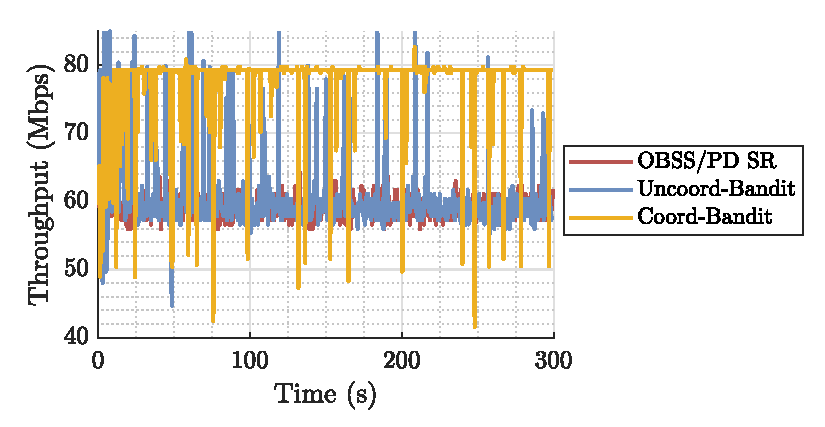
\includegraphics[width=\columnwidth]{figures/dcf_vs_egreedy_new.eps}
\caption{Average throughput observed in the toy scenario for OBSS/PD SR, uncoordinated bandit with $\varepsilon$-greedy, and coordinated bandit with $\varepsilon$-greedy (\texttt{AVG}).}
\label{fig:bandits_performance_toy_scenario}
\end{figure}

\begin{table*}[ht!]
\centering
\caption{Selected actions by uncoordinated (Uncoord-Bandit) and coordinated bandits (Coord-Bandit) in the toy scenario.}
\label{tab:selected_actions_toy_scenario}
\resizebox{.7\textwidth}{!}{%
\begin{tabular}{@{}cccccccc@{}}
\toprule
\multirow{2}{*}{} & \multirow{2}{*}{\textbf{\begin{tabular}[c]{@{}c@{}}Uncoord-Bandit\\ ($\varepsilon$-greedy)\end{tabular}}} & \multicolumn{3}{c}{\textbf{Coord-Bandit ($\varepsilon$-greedy)}} & \multicolumn{3}{c}{\textbf{Coord-Bandit (Thompson sampling)}} \\ \cmidrule(l){3-8} 
 &  & \texttt{AVG} & \texttt{MAX-MIN} & \texttt{PF} & \texttt{AVG} & \texttt{MAX-MIN} & \texttt{PF} \\ \midrule
\textbf{$A_1$} & 4.51\% & 92.49\% & 2\% & 92.48\% & 60.47\% & 58.43\% & 58.43\% \\
\textbf{$A_2$} & 1.67\% & 2.42\% & 2.33\% & 2.75\% & 8\% & 10.85\% & 10.85\% \\
\textbf{$A_3$} & 1.67\% & 2.34\% & 5.75\% & 2.33\% & 8\% & 6.59\% & 6.59\% \\
\textbf{$A_4$} & 92.15\% & 2.75\% & 89.89\% & 2.42\% & 27.58\% & 24.12\% & 24.12\% \\ \bottomrule
\end{tabular}%
}
\end{table*}

As shown in Figure~\ref{fig:bandits_performance_toy_scenario}, the coordinated MABs allow for maximizing the average performance when compared to OBSS/PD SR and uncoordinated bandits. This is because the coordinated mechanism drives the two BSSs playing $A_1$ most of the time (see Table~\ref{tab:selected_actions_toy_scenario}), which matches with the optimal configuration shown in Figure~\ref{fig:toy_scenario}. In contrast, OBSS PD SR statically uses the same configuration and the uncoordinated MABs get stuck in the most conservative action ($A_4$), as a result of the competition among the two BSSs. This effect was previously shown in~\cite{wilhelmi2019collaborative} and occurs when optimal actions lead to poor performance when the other agent selects a different action. As a result, agents using the \texttt{SELF} reward get stuck in a weak equilibrium by conservatively selecting $A_4$. This result motivates the adoption of cooperative strategies.

Still considering the toy scenario (Figure~\ref{fig:toy_scenario}), we study the performance achieved when using different action-selection strategies $\mathcal{E}$ ($\varepsilon$-greedy and Thompson sampling) and shared rewards $\mathcal{R}$ (\texttt{AVG}, \texttt{MAX-MIN}, and \texttt{PF}). For each combination, we show the mean average throughput (including the performance experienced in the transitory phase) of the two BSSs (Figure~\ref{fig:comparison_of_policies}), and the mean throughput evolution (Figure~\ref{fig:comparison_of_policies_temporary_throughput}).

\begin{figure}[ht!]
\centering
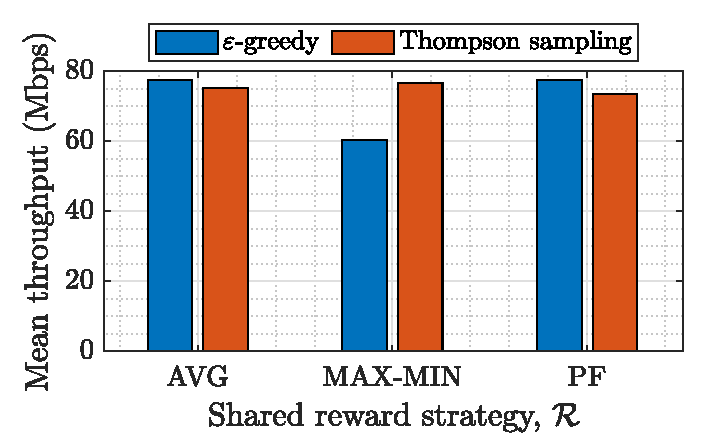
\includegraphics[width=.75\columnwidth]{figures/comparison_of_policies.eps}
\caption{Mean average throughput observed in the toy scenario for $\mathcal{E} = \{\varepsilon\text{-greedy}, \text{Thompson sampling}\}$ and $\mathcal{R} = \{\texttt{AVG}, \texttt{MAX-MIN}, \texttt{PF}\}$.}
\label{fig:comparison_of_policies}
\end{figure}

\begin{figure}[ht!]
\centering
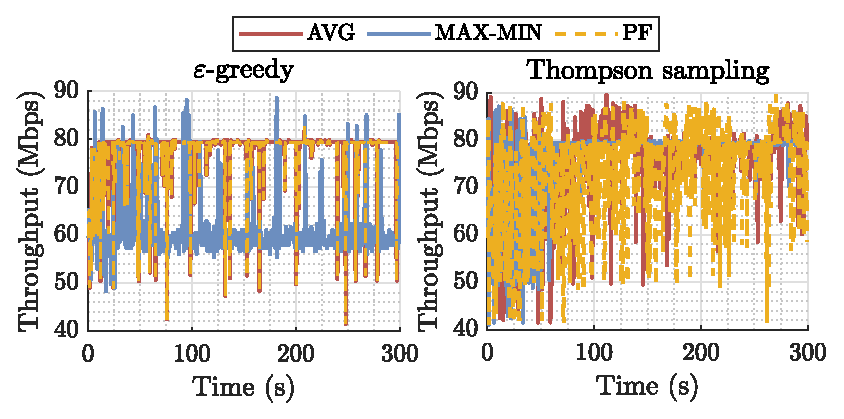
\includegraphics[width=\columnwidth]{figures/comparison_of_policies_temporary_throughput.eps}
\caption{Average throughput observed in the toy scenario when applying $\varepsilon$-greedy (left) and Thompson sampling (right), for $\mathcal{R} = \{\texttt{AVG}, \texttt{MAX-MIN}, \texttt{PF}\}$.}
\label{fig:comparison_of_policies_temporary_throughput}
\end{figure}

As shown in Figure~\ref{fig:comparison_of_policies}, $\varepsilon$-greedy leads to better performance than Thompson sampling when \texttt{AVG} and \texttt{PF} are used. Figure~\ref{fig:comparison_of_policies_temporary_throughput} shows that this is because Thompson sampling explores much more intensively than the considered $\varepsilon$-greedy implementation. Under \texttt{MAX-MIN}, $\varepsilon$-greedy reaches the weak equilibrium mentioned above because \texttt{MAX-MIN} excessively penalizes unfair global configurations, even if those include the best action ($A_1$) by one of the agents. Thompson sampling, in contrast, overcomes this issue thanks to the probabilistic reward models built on top of each action, which allows selecting $A_1$ more times than $\varepsilon$-greedy. The previous observations are reinforced by the results in Table~\ref{tab:selected_actions_toy_scenario}, where $A_1$ ends up being the most played action by Thompson sampling, even for \texttt{MAX-MIN}. However, unlike for $\varepsilon$-greedy (\texttt{AVG} and \texttt{PF}), $A_4$ is also significantly played by Thompson sampling during the transitory phase, i.e., during the first $100$~seconds of the simulation, thus affecting the overall performance in that period.

\subsection{Random scenarios}

Next, we provide more insights into the different considered cooperative strategies by simulating the performance of various BSSs at larger and denser random deployments. For that, we consider the scenario shown in Figure~\ref{fig:randm_scenario}, where $9$~BSSs are deployed in a $3\times 3$ grid of side $D_{sce}=20$~m. Each AP is deployed deterministically in the center of each cubicle and their associated STAs ($1$ per AP) are randomly deployed around their APs within a coverage area with diameter $D_{cov}=3$~m. A frequency reuse $F_R = 3$ means that each BSS is allocated with a random non-overlapping 20~MHz channel from $\mathcal{C} = \{1,2,3\}$. $R=100$ random drops are considered.

\begin{figure}[ht!]
    \centering
    \includegraphics[width=\linewidth]{figures/random_scenario.pdf}
    \caption{Considered 9-BSS random deployment.}
    \label{fig:randm_scenario}
\end{figure}

Figure~\ref{fig:bar_plot_mean_performance_all} shows the mean performance achieved by the OBSS/PD SR baseline and each coordinated algorithm using the different shared reward strategies. In particular, we show the mean values obtained across all devices in the scenario throughout all the simulated random drops, in terms of throughput, access delay, airtime, and time spent in virtual carrier sensing, referred to as the Network Allocation Vector (NAV) time. In all the cases, we display the mean, minimum, and maximum performance experienced across the $9$ BSSs of each simulated deployment.

\begin{figure*}[ht!]
    \centering
    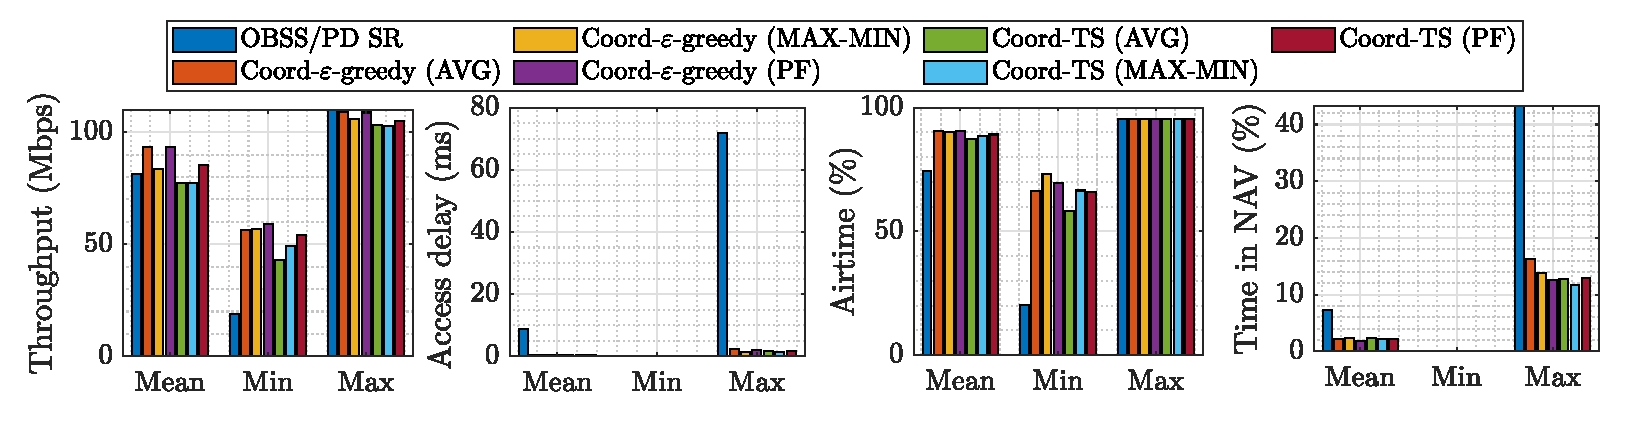
\includegraphics[width=.95\linewidth]{figures/bar_plot_mean_performance_all_new.eps}
    \caption{Mean performance achieved in the $9$-BSS deployment by $\mathcal{E} = \{\varepsilon\text{-greedy}, \text{Thompson sampling}\}$ and $\mathcal{R} = \{\texttt{AVG}, \texttt{MAX-MIN}, \texttt{PF}\}$. Left: throughput, left-center: average delay, right-center: airtime, right: NAV time.}    \label{fig:bar_plot_mean_performance_all}
\end{figure*}

Starting with throughput, we observe that the coordinated MAB implementations slightly improve the mean performance (up to $15$\% for Coord-$\varepsilon$-greedy-\texttt{AVG}) but lead to slightly lower maximum performance (up to $-6$\% for Coord-TS-\texttt{MAX-MIN}). However, the minimum performance of OBSS/PD SR is significantly outperformed by all MAB implementations (up to $210$\% for Coord-$\varepsilon$-greedy-$\texttt{PF}$), which evidences the lack of fairness experienced by the OBSS/PD SR (some BSSs starve) and the potential of coordinated MAB to address this. The same effects are noticed for the rest of the performance metrics. In particular, we notice a great advantage in terms of maximum access delay, which for OBSS/PD SR reaches, on average, $58$~ms, while for the different MAB implementations, it is kept under $3$~ms. This is translated into the minimum airtime experienced by starved devices, which with coordinated MAB enjoy up to $73$\% airtime. Another important metric is the NAV time, which prevents devices from accessing the medium when receiving Ready-to-Send (RTS) and Clear-to-Send (CTS) frames from other overlapping BSSs. Inversely to the airtime, the maximum NAV time is substantially decreased by the coordinated MABs when compared to the OBSS/PD SR. Finally, with respect to the different policies adopted, we observe a similar trend as in the previously described toy scenario. When using $\varepsilon$-greedy, the best-performing reward-sharing strategies are \texttt{AVG} and \texttt{PF}. Nevertheless, \texttt{MAX-MIN} is useful to improve the minimum throughput across the OBSS. As for Thompson sampling, the behavior is slightly different, due to its different approach to handling exploration. In that case, \texttt{PF} is shown to be the best-performing option.

Based on previous observations, we focus on the performance achieved by the best-performing options for coordinated bandits, namely $\varepsilon$-greedy (\texttt{AVG}) and Thompson sampling (\texttt{PF}). Figure~\ref{fig:cdf_mean_throughput_best} shows the Cumulative Distribution Function (CDF) of the mean throughput and channel access delay experienced throughout all the simulations. The two MAB implementations grant higher throughput than OBSS/PD SR,  $\varepsilon$-greedy (\texttt{AVG}) being the best one (Figure~\ref{fig:cdf_mean_throughput_best}). In some cases, OBSS/PD SR leads to slightly higher throughput than Thompson sampling (\texttt{PF}), but this stems from the unfair situations observed above. For mean access delay, the two MAB implementations lead to similar results, but in both cases OBSS/PD SR is substantially outperformed.

\begin{figure}[t!]
    \centering
    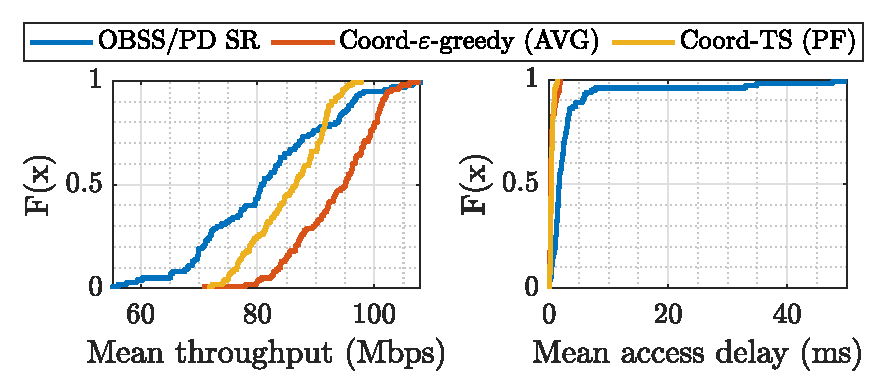
\includegraphics[width=\linewidth]{figures/cdf_mean_throughput_best_new.eps}
    \caption{CDF of the mean throughput (left) and the access delay (right) achieved in the $9$-BSS deployment by OBSS/PD SR, Coord-$\varepsilon$-greedy (\texttt{AVG}) and Coord-TS (\texttt{PF}).}
    \label{fig:cdf_mean_throughput_best}
\end{figure}